\documentclass[12pt,landscape,a4paper]{article}

\usepackage{multicol}
\usepackage{calc}
\usepackage{ifthen}
\usepackage[landscape]{geometry}
\usepackage{amsmath,amsthm,amsfonts,amssymb}
\usepackage{color,graphicx,overpic}
\usepackage{hyperref}
\usepackage[table]{xcolor}

\usepackage{minted}

\usepackage{circuitikz}
\usetikzlibrary{calc}




% This sets page margins to .5 inch if using letter paper, and to 1cm
% if using A4 paper. (This probably isn't strictly necessary.)
% If using another size paper, use default 1cm margins.
\ifthenelse{\lengthtest { \paperwidth = 11in}}
    { \geometry{top=.5in,left=.5in,right=.5in,bottom=.5in} }
    {\ifthenelse{ \lengthtest{ \paperwidth = 297mm}}
        {\geometry{top=1cm,left=1cm,right=1cm,bottom=1cm} }
        {\geometry{top=1cm,left=1cm,right=1cm,bottom=1cm} }
    }

% Turn off header and footer
\pagestyle{empty}

% Redefine section commands to use less space
\makeatletter
\renewcommand{\section}{\@startsection{section}{1}{0mm}%
                                {-1ex plus -.5ex minus -.2ex}%
                                {0.5ex plus .2ex}%x
                                {\normalfont\large\bfseries}}
\renewcommand{\subsection}{\@startsection{subsection}{2}{0mm}%
                                {-1explus -.5ex minus -.2ex}%
                                {0.5ex plus .2ex}%
                                {\normalfont\normalsize\bfseries}}
\renewcommand{\subsubsection}{\@startsection{subsubsection}{3}{0mm}%
                                {-1ex plus -.5ex minus -.2ex}%
                                {1ex plus .2ex}%
                                {\normalfont\small\bfseries}}
\makeatother

% Define BibTeX command
\def\BibTeX{{\rm B\kern-.05em{\sc i\kern-.025em b}\kern-.08em
    T\kern-.1667em\lower.7ex\hbox{E}\kern-.125emX}}

% Don't print section numbers
\setcounter{secnumdepth}{0}


\setlength{\parindent}{0pt}
\setlength{\parskip}{0pt plus 0.5ex}

%My Environments
\newtheorem{example}[section]{Example}
% -----------------------------------------------------------------------

\begin{document}
\raggedright
\footnotesize
\begin{multicols}{4}

\begin{minipage}[t]{\linewidth}
\rowcolors{2}{gray!25}{white}
\begin{tabular}{l | l | l}
    Bit & Decimal & Hex \\
    0 & 1 & 1 \\
    1 & 2 & 16 \\
    2 & 4 & 256 \\
    3 & 8 & 4096 \\
    4 & 16 & 65.536 \\
    5 & 32 & Hex \\
    6 & 64 & Hex \\
    7 & 128 & Hex \\
    8 & 256 & Hex \\
    9 & 512 & Hex \\
    10 & 1024 & Hex \\
    11 & 2048 & Hex \\
    12 & 4096 & Hex \\
    13 & 8192 & Hex \\
    14 & 16.384 & Hex \\
    15 & 32.768 & Hex \\
    16 & 65.536 & Hex \\
\end{tabular}

\begin{tabular}{l | l | l}
    Binary & Decimal & Hex \\
    0000 & 0 & 0 \\
    0001 & 1 & 1 \\
    0010 & 2 & 2 \\
    0011 & 3 & 3 \\
    0100 & 4 & 4 \\
    0101 & 5 & 5 \\
    0110 & 6 & 6 \\
    0111 & 7 & 7 \\
    1000 & 8 & 8 \\
    1001 & 9 & 9 \\
    1010 & 10 & a \\
    1011 & 11 & b \\
    1100 & 12 & c \\
    1101 & 13 & d \\
    1110 & 14 & e \\
    1111 & 15 & f \\
\end{tabular}

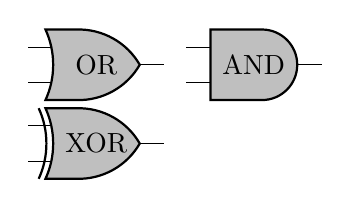
\begin{tikzpicture}

    % Circuit style
    \ctikzset{
        logic ports=ieee,
        logic ports/scale=0.8,
        logic ports/fill=lightgray
    }
    
    % Logic ports
    \node[or port] (OR) at (0,1){OR};
    \node[and port] (AND) at (2,1){AND};
    \node[xor port] (XOR) at (0,0){XOR};
\end{tikzpicture}

$50 mod 3$ → $50/3 = 16.6667$ \\
→ $16.6667 - 16 = 0.6667$ \\
→ $0.6667 * 3 = 2$

lw → longest insn.
\end{minipage}

\begin{tiny}
\begin{minted}{verilog}
    module coffee_mealy(
        input clk,
        input reset,
        input insert,
        input [1:0] coins,
        output reg coffee,
        output [2:0] state_display
        );
        
        localparam STAT0 = 0,
        STAT1 = 1,
        STAT2 = 2;
            
        localparam COIN0 = 2'b00,
            COIN1 = 2'b10,
            COIN2 = 2'b01;
            
        
        reg insert_prv;
        reg [2:0] state_next;
        reg [2:0] state_curr;
        reg coffee_next;
        
        assign state_display = state_curr;
    
        
        //reset active HIGH
        //transition on: insert HIGH && clock edge
        //Update output on: posedge clk
        
        //Initial state -> coins is 0
        always @(posedge clk) begin
            //Reset?
            if(reset) begin
                insert_prv <= 1'b0;
                coffee <= 1'b0;
                state_curr <= 1'b0;
            end
            else if (insert && ~insert_prv) begin
                insert_prv <= insert;
                state_curr <= state_next;
                coffee <= coffee_next;
            end
            else begin
                insert_prv <= insert;
                state_curr <= state_curr;
                coffee <= coffee;
            end
        end
    \end{minted}
\end{tiny}
\begin{tiny}
\begin{minted}{verilog}
$display : print the immediate values
$strobe : print the values at the end of the current timestep
$monitor : print the values at the end of the current timestep if any values changed. 
$monitor can only be called once; sequential call will override the previous.
$write : same as $display but doesn't terminate with a newline (\n) 
$display("display a:%h b:%h @ %0t", a, b, $time);

%d -> decimal %t -> time %h -> hex %b -> binary %f -> real %c -> char %s -> string

$finish(1) -> Exit + Prints simulation time and location 
$time -> Scaled Time Integer
$stime -> Scaled Time Real
\end{minted}
\end{tiny}
\columnbreak
\begin{tiny}
\begin{minted}{verilog}
    always @(*) begin
    case (state_curr)    
        STAT1: begin
            case (coins)
            COIN1: begin
                state_next = STAT2;
                coffee_next = 0;
            end
            COIN2: begin 
                state_next = STAT0;
                coffee_next = 1;
            end
            default: begin 
                state_next = STAT1;
                coffee_next = 0;
            end
            endcase
        end
        
        STAT2: begin
            case (coins)
            COIN1: begin
                state_next = STAT0;
                coffee_next = 1;
            end
            COIN2: begin 
                state_next = STAT1;
                coffee_next = 1;
            end
            default: begin 
                state_next = STAT2;
                coffee_next = 0;
            end
            endcase
        end
        
        //State 0
        default: begin
            case (coins)
            COIN1: begin
                state_next = STAT1;
                coffee_next = 0;
            end
            COIN2: begin 
                state_next = STAT2;
                coffee_next = 0;
            end
            default: begin 
                state_next = STAT0;
                coffee_next = 0;
            end
            endcase
        end
    endcase
end  
endmodule

assign out = out_next; // For fast changes
\end{minted}
\end{tiny}
\columnbreak

\subsection{Isns Reg Order}
add rd, rs1, rs2\\
bne rs1, rs2, IMM

\begin{minipage}[t]{\linewidth}
\rowcolors{2}{gray!25}{white}
\begin{tabular}{l | l }
    ns & MHz \\
    1 & 1000 \\
    10 & 100 \\
    100 & 10 \\
    1000 & 1 \\
\end{tabular}
\subsection{Twos compliment}
\begin{tabular}{l}
1. Make it bin $5 = 0101$\\
2. NOT it $1010$\\
3. Add 1 $1011$\\
4. fill out with 1\'s $11111111011$\\
\end{tabular}
\end{minipage}



\end{multicols}
\subsection*{Cache Timing}
\rowcolors{2}{gray!25}{white}
\begin{tabular}{l}
    CPI = average number of cycles per instruction; \\
    $T_{exec}$ = $N_{instr}$ x $CPI$ x $T_{cycle}$;\\
    CPI = $CPI_{ideal}$ + $CPI_{stall}$;\\
    For pipelined processor: $CPI_{ideal}$ = 1;\\
    $CPI_{stall}$ = \%reads x miss\_rate\_read x mis\_spenalty\_read + \%writes x miss\_rate\_write x miss\_penalty\_write; \\
    Cache misses increase CPI by adding stall cycles;\\
    Averge Memory access time = Time for a hit + Miss rate x Miss penalty\\
\end{tabular}

\subsection*{Cache Addressing}
\begin{tabular}{l}
    Address\_size = N\_tag\_bits + N\_index\_bits + N\_word\_offset\_bits + Byte\_offset;\\
    $N\_blocks\_in\_cache = 2^{N\_index\_bits}$;\\
    $N\_word\_in\_block = log_2(words)$;\\
    Direct\_memory → associativity = 1;\\
    Cache\_size = N\_blocks\_in\_cache * associativity * (N\_bits\_in\_word * N\_words\_in\_block + N\_tag\_bits + Valid\_bit + dirty\_bit);\\
\end{tabular}

\includegraphics[scale=0.6]{floating.jpg}
\includegraphics[scale=0.3]{direct-two-ass.PNG}
\includegraphics[scale=0.3]{offset.PNG}
\multicols {3}
\begin{tiny}
\begin{minted}{verilog}
`timescale 1ns / 1ps
module custom_counter_v1_0_tb();
  //stuff you need
   reg arstn = 1'b0;
   reg [2:0] write_prot = 3'd0;    //type of write(leave at 0)
   reg write_addr_valid = 1'b0;    //master indicating address is valid
   custom_counter_v1_0 #(
       .number_of_clk_cycles(10)    //custom wires
   ) custom_counter_v1_0_inst (
   // Define wires
       .leds(leds),
   );
   always 
   #5 aclk <= ~aclk;
   initial 
   begin
   arstn = 0;
   #20 arstn = 1;
   axi_write(32'd4,1'b1);
   axi_read(32'd8, output_data);
   #200
   $finish; 
   end
   // TASKS
   task axi_read;
   input [31:0] addr; //Defines here
   output reg [31:0] data;
   begin
       #3 read_addr <= addr; //puts adress on the bus
       read_addr_valid <= 1'b1; //indicating address is valid
       read_data_ready <= 1'b1; //indicting ready for a response
       wait(read_addr_ready); //wait till slave is ready to read the address
       @(posedge aclk); //handshake occurs
       read_addr_valid <= 1'b0;
       wait(read_data_valid);
       @(posedge aclk);
       data <=read_data;
       @(posedge aclk);
       read_data_ready <= 1'b0;
   end
   endtask
endmodule
    \end{minted}
\end{tiny}


\end{document}
